\documentclass[tikz, border=10pt]{standalone}
\usetikzlibrary{positioning, calc, backgrounds, shapes.geometric}

\begin{document}
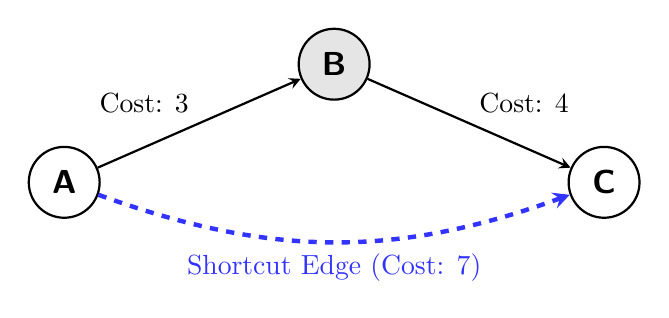
\begin{tikzpicture}[
    node distance=2.5cm,
    vertex/.style={circle, draw, thick, minimum size=0.9cm, inner sep=1pt, font=\sffamily\large\bfseries},
    directed/.style={->, >=stealth, thick},
    shortcut/.style={->, >=stealth, ultra thick, dashed, draw=blue!80}
]
    % Nodes
    \node[vertex] (A) {A};
    \node[vertex, right=of A, yshift=1.5cm, fill=gray!20] (B) {B};
    \node[vertex, right=of B, yshift=-1.5cm] (C) {C};

    % Original Edges
    \draw[directed] (A) -- node[above left] {Cost: 3} (B);
    \draw[directed] (B) -- node[above right] {Cost: 4} (C);

    % Shortcut Edge
    \draw[shortcut] (A) to[bend right=20] node[below, text=blue!80] {Shortcut Edge (Cost: 7)} (C);
\end{tikzpicture}
\end{document}